\documentclass[12pt, letterpaper]{article}
\usepackage{draftwatermark}
\usepackage[spanish]{babel}
\usepackage{graphicx}
\usepackage{parskip}
\usepackage{enumitem}
\usepackage{transparent}

% Document Settings
\setlength{\parindent}{0cm}
\setlength{\parskip}{4mm}
\setlist{nosep}
\renewcommand{\familydefault}{\sfdefault}
\SetWatermarkText{
    {\transparent{0.05}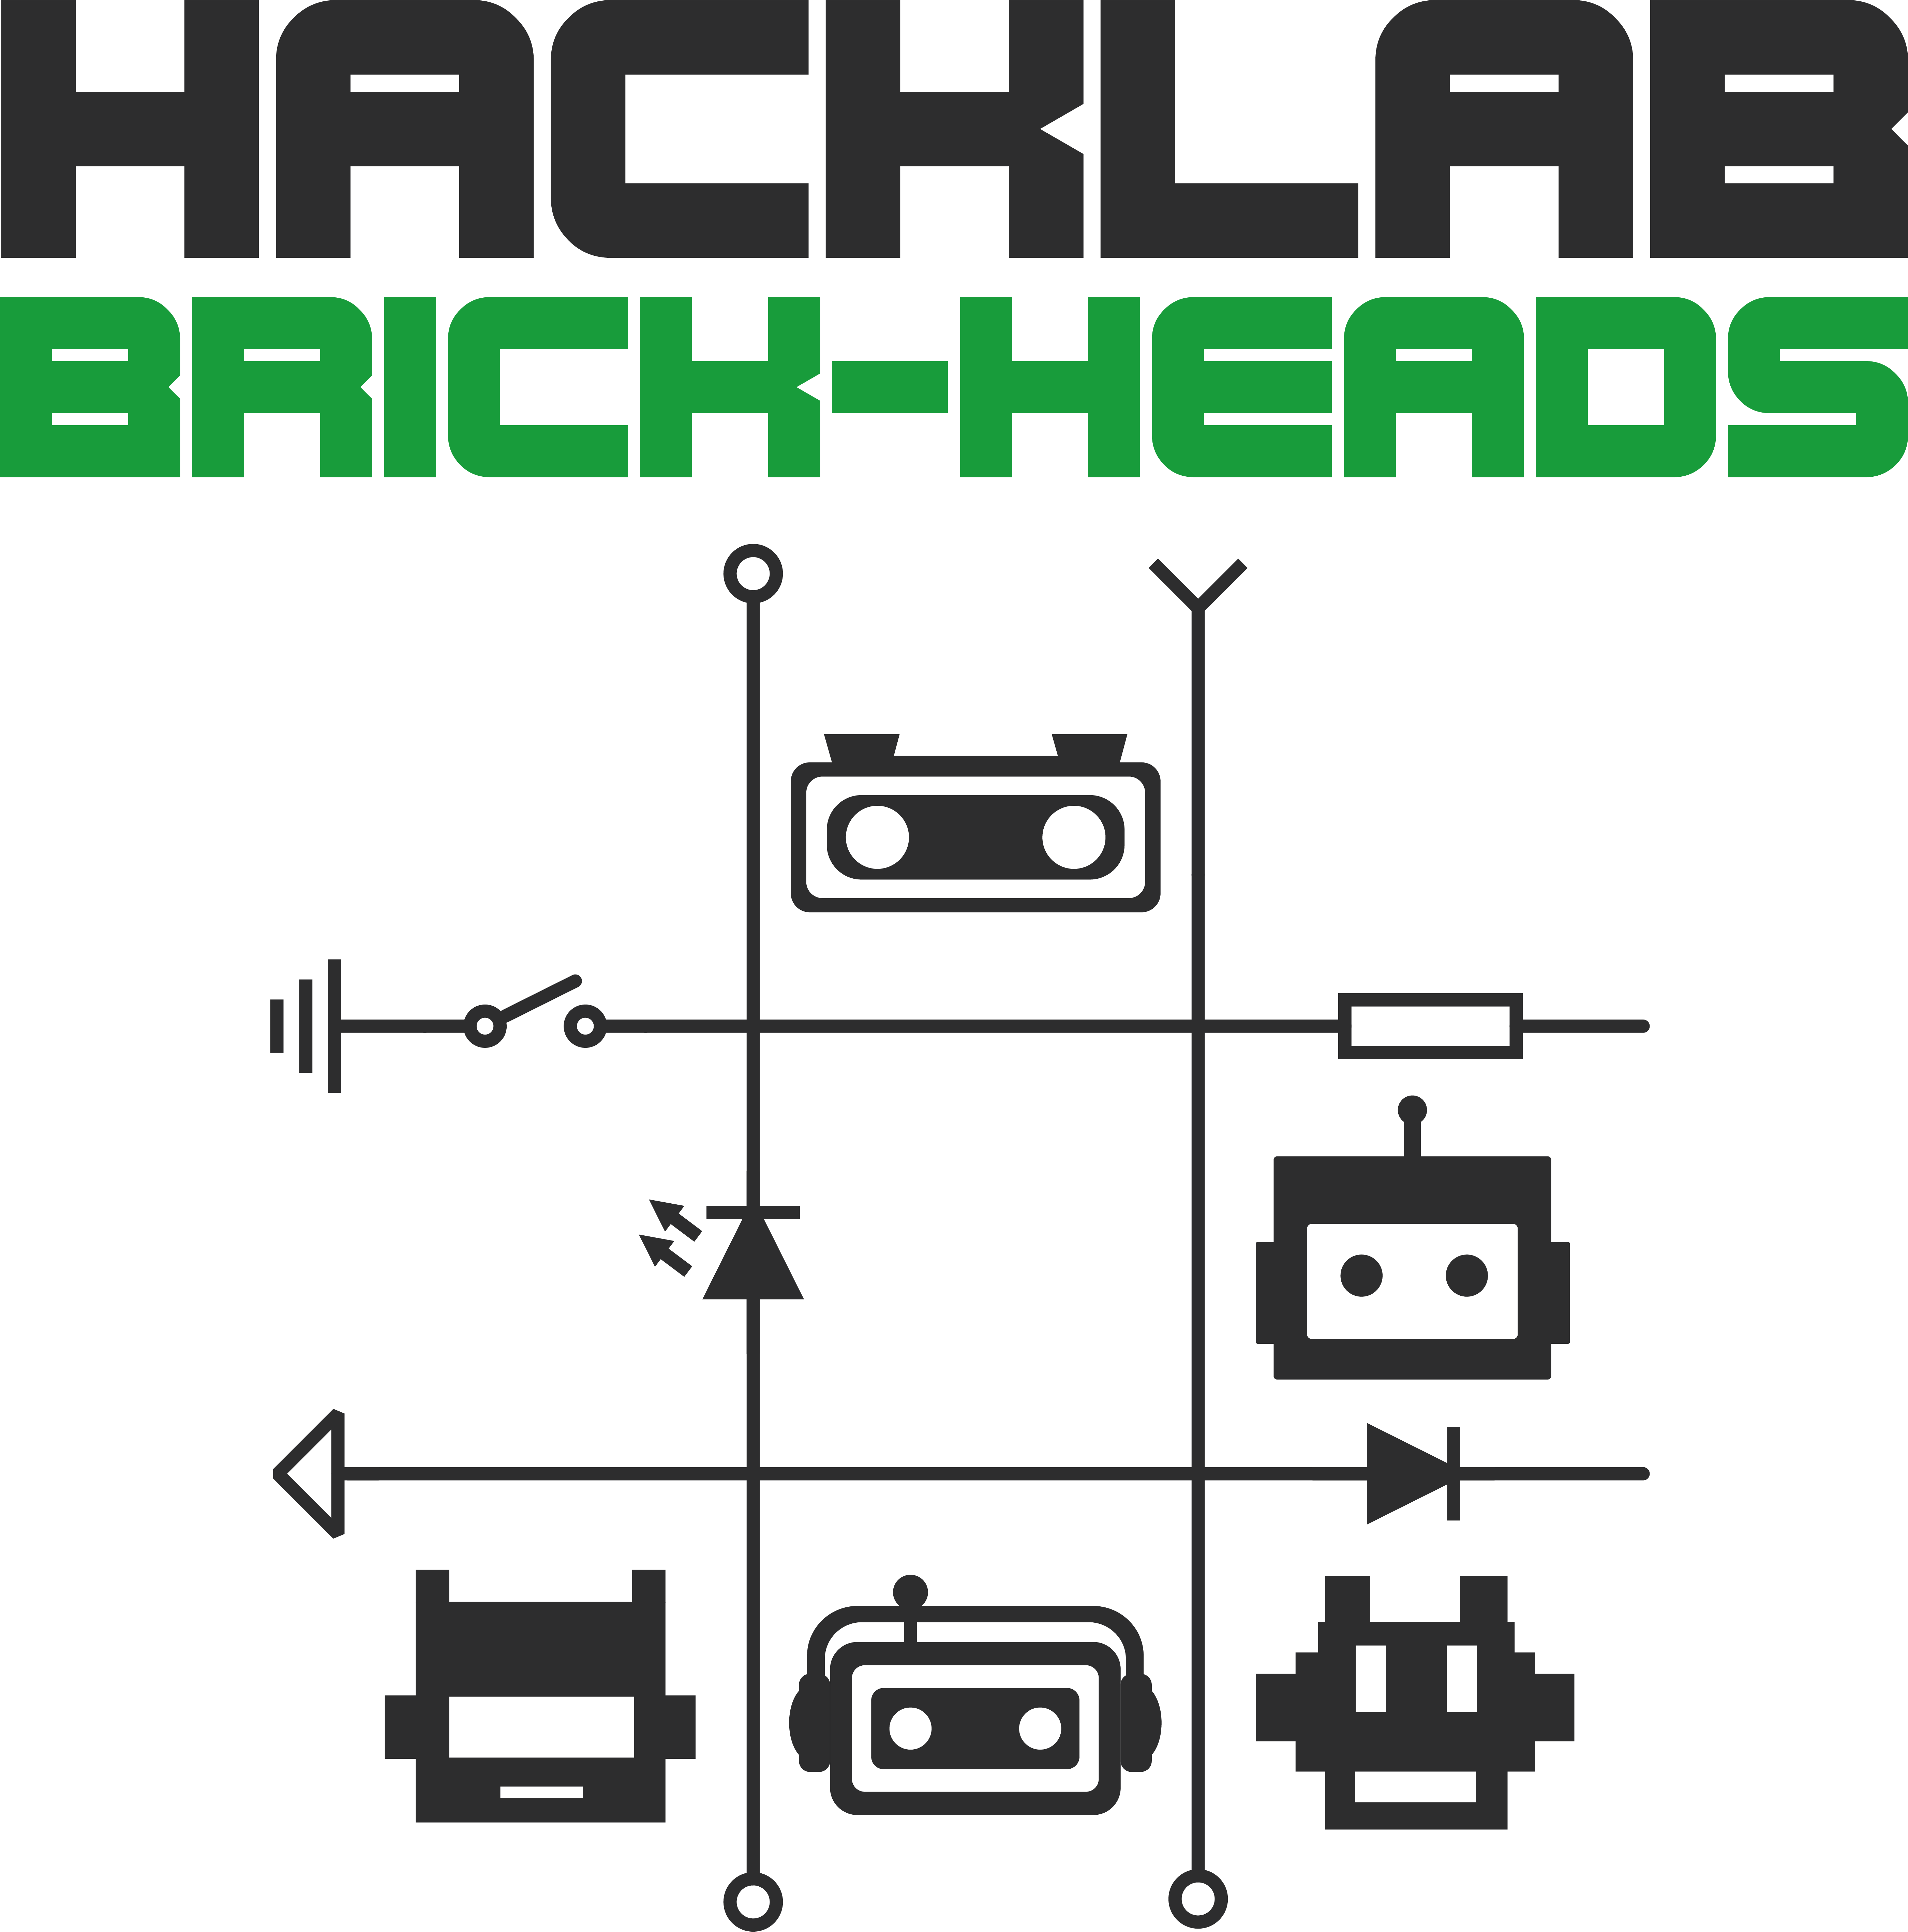
\includegraphics[width=16cm]{./images/square_dark.png}}    
}
% \SetWatermarkScale{5}
\SetWatermarkColor[gray]{0.1}
\SetWatermarkAngle{0}

% Metadata
\title{Reglamento Interno ``HackLab BrickHeads''}
\author{Versión I}
\date{Febrero 2023}


% Document
\begin{document}
    \maketitle
    % \hspace{1cm}

    \begin{center}
        HackLab BrickHeads es un espacio Hacker de conocimiento abierto, 
        experimentación y aprendizaje colectivo
    \end{center}

    Nuestros principales pilares son:
    \begin{itemize}
        \item \textbf{T}ecnología
        % no es posible concebir un mundo sin este 
        % pilar y volver al pasado no es la respuesta a nuestros problemas 
        % actuales, la tecnología es un medio que debe garantizar principalmente 
        % nuestro calidad de vida.
        \item \textbf{E}ducación
        % si bien la educación no es el único pilar que 
        % garantiza una vida más plena, mayores oportunidades y calidad de vida 
        % en general, es muy importante ya que no se da solamente en la escuela, 
        % la universidad o centros de formación académica, se da tambien en casa, 
        % entre vecinos; en sociedad. Por ende es un factor que debe garantizarse 
        % desde edades tempranas, en ese sentido, toda persona es un maestro. ¿Qué 
        % tan bueno? eso debe atenderse desde la individualidad.
        \item \textbf{C}ultura/\textbf{C}iencia
        \item \textbf{S}ociedad
    \end{itemize}

\section{MANIFIESTO}
    El conocimiento es un pilar fundamental del desarrollo humano, es libre y no
    debería privarse.

    La tecnología es un medio, mas no el fin. Es una herramienta de las muchas 
    para la transformación y evolución a una sociedad mejor.

    La privacidad, la seguridad y los datos personales son derechos humanos
    fundamentales.

    La colaboración, contribución y participación abierta son clave para el
    desarrollo de tecnología con conciencia y responsabilidad social.

    Es importante fomentar la inclusión y diversidad en todos los aspectos.

    Nada es absolutamente cierto, ni absolutamente falso, las respuestas más
    interesantes se encuentran en el terreno de lo matizado.

    Debemos manejar, enseñar y difundir tecnología de forma crítica y reflexiva.

    \section{DE LOS INTEGRANTES}
    Todo integrante de HackLab BrickHeads es parte fundamental de la 
    comunidad, sin importar cualquier elemento diferenciador, todos los miembros 
    tiene el mismo nivel de importancia, beneficios y responsabilidad.

    \subsection{Estructura Organizativa}
    HackLab BrickHeads tiene una estructura organizativa que se 
    utiliza netamente para interactuar con el exterior o para la toma de 
    decisiones críticas, estas son algunas situaciones:

    \begin{itemize}
        \item Contactar y coordinar proyectos con comunidades, organizaciones u 
        otras externas.
        \item Toma de decisiones rápidas y críticas.
        \item Como representante ante cualquier eventualidad externa
        \item Organización de proyectos y actividades generales.
    \end{itemize}

    Fuera de esas situaciones HackLab BrickHeads se considera una comunidad 
    sin estructura organizativa.

    El único rol ante las eventualidades planteada anteriormente es el/la
    \textbf{Lider de comunidad}, cuyas responsabilidades son:
    \begin{itemize}
        \item Promover la camaradería y tranquilidad dentro de la comunidad.
        \item Representar al HackLab BrickHeads ante eventualidades.
        \item Mediar opiniones, proyectos, ideas, acuerdos, desacuerdos u otros 
        internamente. 
        \item Asistir a cada miembro en la medida de sus posibilidades.
        \item Respetar, exponer y manejar los matices dentro de una lluvia de
        ideas, reuniones u otras.
        \item Orientar toda situación hacia un panorama de sinergia.
        \item Debe transmitir de forma transparente toda información concerniente 
        a la comunidad.
    \end{itemize}

    Por otro lado, HackLab BrickHeads tiene responsabilidades internas que 
    confluyen conformando roles eventuales, es decir, que pueden ser cubiertos 
    por cualquiera de los miembros de la comunidad.
    \begin{itemize}
        \item Relaciones Sociales
        \item Gestión de actas
        \item Diseño e Imagen
        \item Manejo de fondos
    \end{itemize}

    La comunidad cree firmemente que una estructura jerárquica convencional no
    es necesaria cuando se tiene miembros proactivos, automotivados y
    sinérgicos.

    \subsection{Beneficios}
    Todo miembro del HackLab BrickHeads tiene como beneficios:
    \begin{itemize}
        \item Mentoría por parte de cada uno de los miembros (de parte del 
        miembro idóneo para tal mentoría).
        \item Ventana de oportunidades. Tus ideas, proyectos u otros son 
        importantes, si el HackLab BrickHeads tiene las posibilidades 
        de hacerlas visibles siempre sucederá, cualquier propuesta externa 
        hacia el HackLab BrickHeads para el crecimiento para cada uno de sus
        miembros siempre será socializada adecuadamente.
        \item No te quedes con la duda. En el HackLab BrickHeads siempre tendrás
        un espacio para compartir cualquier idea, duda, pregunta u otras, por 
        más alocadas que parezcan.
        \item Ser líder de proyecto. Todo proyecto que plantees, socializado y 
        aceptado por lo miembros del HackLab BrickHeads te vuelve un líder 
        de proyecto, responsable principal y representante de tal proyecto.
    \end{itemize}

    \subsection{Deberes}
    Los deberes de todo miembro son:
    \begin{itemize}
        \item Promover la camaradería y tranquilidad dentro de la comunidad.
        \item Apoyar a los demás miembros en la medida de sus posibilidades.
        \item Respetar las ideas, pensamientos, dudas u otros aspectos 
        personales de cada miembro.
        \item Orientar toda situación hacia un panorama de armonía y 
        entendimiento.
        \item Debe transmitir de forma transparente toda información 
        concerniente a la comunidad.
        \item Demostrar puntualidad y responsabilidad.
    \end{itemize}
    
    \subsection{Sanciones}
    Existen dos categorías de sanciones:
    \begin{itemize}
        \item \textbf{Leve}. Llamada de atención por parte de unos de los
        miembros de la comunidad.
        \item \textbf{Grave}. Suspensión de membresía, con tiempo a evaluarse a 
        través de una reunión general.
    \end{itemize}

    \subsubsection{Sanción Leve}
    Se consideran sanciones leves:
    \begin{itemize}
        \item Faltar el respeto a un o varios miembros de la comunidad.
        \item Utilizar o actuar en nombre de la comunidad sin consensuarlo.
        \item Ocultar información o brindar información crítica a terceros.
        \item No respetar la diversidad e ir en contra de la inclusión con 
        respecto a miembros, postulantes o personas en general.
    \end{itemize}

    Tres sanciones leves son equivalentes a una Sanción Grave.

    \subsubsection{Sanción Grave}
    Se consideran sanciones graves:
    \begin{itemize}
        \item Utilizar la tecnología para comprometer la privacidad y datos 
        personales de terceros en nombre de la comunidad o para beneficio 
        propio. 
        \item Comprometer el nombre del HackLab BrickHeads para beneficios 
        propios o de terceros.
        \item Lucrar de forma no consensuada a través de la comunidad.
        \item Hacer uso indebido de los recursos de la comunidad.
    \end{itemize}

    \section{ÁREAS DE TRABAJO}
    El HackLab BrickHeads desde su inicio siempre tuvo una inclinación hacía la 
    electrónica, robótica y programación con impacto social, sin embargo, han 
    sido áreas determinadas por el contexto y las necesidades del momento.
    
    Las áreas fuertes dentro de la comunidad están determinadas por sus miembros 
    en la actualidad dichas áreas son:
    \begin{itemize}
        \item Robótica
        \item Electrónica
        \item Automatización Web
        \item Inteligencia Artificial
        \item Programación
        \item Linux
        \item Movimiento al rededor del FLOSS (Free/Libre and Open Source 
        Software).
    \end{itemize}
    
    \section{TERMINOLOGÍA}
    \begin{itemize}
        \item \textbf{Hacker}, es una persona capaz de usar sus conocimientos 
        especializados y transdimensionales para resolver un problema concreto, 
        en resumen, un Hacker es una persona que tiene dominio de distintas 
        habilidades y las utiliza para resolver desde los problemas más 
        sencillos hasta los más intrincados. Un gran ejemplo es 
        \textit{MacGyver} (personaje ficticio).
    \end{itemize}
\end{document}